\chapter{Renormalisation, naturalité et problème de la hiérarchie}

\lectureoverview{Les idées centrales de ce cours sont nées de questions sur la renormalisation dans le Modèle standard. Nous commencerons donc par le sens physique de la renormalisation : éliminer les degrés de liberté trop petits et trop rapides au regard de la question posée, puis encoder leurs effets dans une description effective. Une molécule en fournit le modèle. L’analyse dimensionnelle prolonge ensuite ce raisonnement à la théorie quantique des champs scalaires, où elle met en évidence la sensibilité quadratique de la masse d’un scalaire, le problème de la hiérarchie associé au champ de Higgs, la protection dont bénéficient les fermions et les bosons de jauge, ainsi que le problème encore bien plus sévère de l’énergie du vide.}

\section{La physique à l’échelle de la question posée}

La plupart des idées que nous développerons ce trimestre sont issues de questions sur la renormalisation---parfois des énigmes, parfois des observations utiles---dans le Modèle standard. La renormalisation associe deux habitudes de pensée. La première consiste à éliminer d’une description les structures à des distances si courtes qu’elles sont sans pertinence pour la question posée. La seconde est l’analyse dimensionnelle, qui permet souvent de déterminer la réponse à courte distance avant même d’évaluer la moindre intégrale difficile.

Cette élimination des détails se produit dans toute la physique. Pour comprendre un noyau, nous pouvons partir des quarks et de la chromodynamique quantique. Après avoir calculé les masses et les spins du proton et du neutron, ainsi que leurs forces nucléaires effectives, nous pouvons, dans bien des cas, oublier leur sous-structure en quarks. Le mouvement nucléaire est suffisamment lent pour qu’une mécanique quantique non relativiste des protons et des neutrons soit souvent une description plus utile.

Au niveau suivant, la physique atomique n’a généralement pas besoin de connaître la constitution interne d’un noyau. La physique nucléaire nous indique quels noyaux et isotopes existent et fournit des propriétés telles que la masse et la charge électrique. Nous repartons alors d’un nouvel ensemble d’objets élémentaires effectifs : les noyaux et les électrons. Les quarks, les protons et les neutrons n’ont pas cessé d’exister ; leurs effets sont condensés dans les paramètres associés aux noyaux.

La quantité de détails conservés dépend de la question suivante. Un calcul atomique peut nécessiter la masse nucléaire, puisqu’elle intervient dans la masse réduite, et il a certainement besoin de la charge, qui détermine le champ coulombien. En général, il n’a pas besoin de savoir quel quark porte telle fraction de l’impulsion du noyau. Il existe environ quatre-vingt-dix charges élémentaires, et davantage d’espèces nucléaires si l’on compte les isotopes. On peut prendre ce catalogue comme donnée d’entrée. Les électrons, en revanche, ne peuvent pas encore être éliminés : leur mouvement est précisément ce qui donne naissance à la structure atomique.

Après avoir résolu le problème atomique, nous pouvons de même considérer les atomes comme les briques constitutives des molécules. La liste fantaisiste de Susskind — atomes de biscuits, atomes de café, atomes de chocolat et atomes de ketchup — fait ressortir une idée sérieuse : à chaque niveau correspond une nouvelle description. Une fois connues les propriétés et les forces moléculaires, on peut assembler les molécules en structures plus grandes, semblables à des constructions en Meccano, sans rouvrir le problème électronique à chaque étape.

Chaque passage d’un niveau à l’autre est un coarse-graining. La nouvelle description peut être moins exacte au sens absolu, mais elle est bien plus utile à l’échelle visée. En théorie quantique des champs, cette question est inévitable, car un champ possède des modes à toutes les longueurs d’onde, y compris arbitrairement courtes. Nous faisons donc la somme des effets des longueurs d’onde trop courtes pour être résolues et les remplaçons par de nouveaux paramètres effectifs. Cette opération, associée à l’analyse dimensionnelle, constitue le contenu physique de la renormalisation.

\section{Une molécule comme modèle}

Considérons deux atomes et cherchons une description simple de leur mouvement relatif. Chaque atome contient un noyau lourd et un nuage d’électrons. Même un proton est environ deux mille fois plus lourd qu’un électron, et les noyaux plus lourds accentuent encore la séparation des échelles. On peut se représenter deux boules de bowling entourées de mouches qui volent rapidement : les noyaux réagissent lentement, tandis que l’état électronique se réorganise vite.

Notons \(R_a\) et \(P_a\) les positions et les impulsions nucléaires, de masse commune \(M\), et \(r_i\) et \(q_i\) les coordonnées et les impulsions des électrons, de masse \(m_e\). En omettant des facteurs usuels tels que \(4\pi\epsilon_0\), le Hamiltonien prend la forme schématique suivante :
\begin{align}
H={}&
\frac{P_1^2}{2M}+\frac{P_2^2}{2M}
+\frac{e^2}{R_{12}}
+\sum_i\frac{q_i^2}{2m_e}
+\frac12\sum_{i\ne j}\frac{e^2}{r_{ij}}
\nonumber\\
&-\sum_i\left(
\frac{e^2}{|R_1-r_i|}
+\frac{e^2}{|R_2-r_i|}
\right).
\label{eq:molecular-hamiltonian}
\end{align}
La première ligne contient les énergies cinétiques nucléaires, leur répulsion coulombienne mutuelle et l’énergie cinétique électronique. La deuxième ligne comprend la répulsion entre électrons et l’attraction entre électrons et noyaux. Pour des noyaux de charges générales, il faut rétablir les facteurs correspondants de \(Z_a\) ; le cours laisse les charges sous forme schématique, car c’est la séparation des échelles de temps qui nous intéresse.

Il existe deux types de mouvement caractéristiques. Les noyaux sont lourds et lents ; les électrons sont assez légers et rapides pour former une sorte de flou. En première approximation, fixons les positions nucléaires et regroupons tous les termes qui dépendent des électrons dans un Hamiltonien électronique,
\begin{equation}
H_{\mathrm{el}}(R_1,R_2).
\end{equation}
Pour chaque configuration nucléaire fixée, résolvons
\begin{equation}
H_{\mathrm{el}}(R_1,R_2)
\psi_0(r_1,\ldots,r_N;R_1,R_2)
=
E_{\mathrm{el}}(R_1,R_2)\psi_0.
\label{eq:electronic-ground-state}
\end{equation}
Nous conservons la plus petite valeur propre électronique. Les électrons n’ont pas été négligés : leur mouvement rapide a été entièrement résumé par la fonction \(E_{\mathrm{el}}(R_1,R_2)\).

Le raisonnement est adiabatique. Pendant un ajustement électronique rapide, les noyaux se déplacent si peu que l’on peut traiter leurs coordonnées comme des paramètres. Une fois le problème aux valeurs propres électroniques résolu, ces mêmes coordonnées peuvent à nouveau évoluer. À chaque configuration qui change lentement, le nuage électronique suit son état fondamental instantané. Un traitement plus précis pourrait conserver les surfaces électroniques excitées et les transitions entre elles, mais la surface dominante suffit déjà à illustrer l’idée de renormalisation.

\begin{figure}[htbp]
\centering
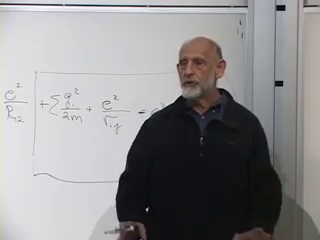
\includegraphics[width=0.72\textwidth]{lecture_01_figure_02.png}
\caption{Le Hamiltonien moléculaire reste au tableau lorsque le problème de l’état fondamental électronique est introduit. La forme saisie dans l’équation ~\eqref{eq:molecular-hamiltonian} rend compte des termes masqués sur cette image.}
\lectureframe{00:16:19}
\end{figure}

\begin{classroomqa}
\audiencequestion{Les impulsions nucléaires sont-elles simplement posées égales à zéro ?\lecturetimestamp{00:15:39}}
\lecturerresponse{Seulement de façon provisoire. Dans l’approximation dominante, on traite les noyaux comme s’ils étaient cloués sur place, car ils se déplacent beaucoup plus lentement que les électrons. Nous réintroduirons leurs impulsions lorsque nous résoudrons le problème nucléaire effectif ; cette approximation ne viole donc pas le principe d’incertitude.}
\end{classroomqa}

L’énergie de l’état fondamental électronique contribue désormais au potentiel ressenti par les noyaux :
\begin{equation}
V_{\mathrm{eff}}(R_1,R_2)
=\frac{e^2}{R_{12}}+E_{\mathrm{el}}(R_1,R_2).
\label{eq:molecular-effective-potential}
\end{equation}
L’invariance par rotation et par translation réduit, pour deux atomes isolés, ce potentiel à une fonction de leur séparation \(R_{12}\). À très courte distance, la répulsion coulombienne nucléaire domine. À très grande distance, l’interaction est faible. Entre ces deux limites, le nuage électronique peut créer une région attractive et un minimum. La fonction d’onde nucléaire se concentre alors près de ce minimum et décrit une molécule liée.

Remarquons l’ordre des opérations. Nous n’avons pas supposé une attraction empirique pour ensuite écarter les électrons. Nous avons d’abord résolu leur problème quantique dans le champ des noyaux fixes. Ce n’est qu’ensuite que nous avons éliminé leurs coordonnées explicites tout en conservant la valeur propre obtenue. La physique à courte distance subsiste dans la forme, la profondeur et la courbure de \(V_{\mathrm{eff}}\). La position de son minimum fixe la distance d’équilibre, sa courbure détermine les petites vibrations et son comportement asymptotique indique si un état lié existe. Une seule fonction effective transporte toute cette information électronique dans le problème plus lent.

Ainsi, un Hamiltonien complexe à plusieurs électrons est devenu un Hamiltonien nucléaire à deux corps doté d’un nouveau potentiel. Nous avons éliminé les degrés de liberté rapides tout en conservant leur effet complet à basse énergie. Le potentiel a été renormalisé. Ce raisonnement familier de Born--Oppenheimer n’est généralement pas présenté sous ce nom, mais il contient précisément l’idée dont nous avons besoin :
\begin{equation}
\begin{gathered}
\text{fast microscopic dynamics}\\
\Downarrow\\
\text{effective parameters for slow dynamics}
\end{gathered}
\end{equation}

\section{Unités naturelles et dimension d’un champ}

En théorie quantique des champs, les modes à éliminer peuvent être décrits de manière équivalente comme des modes à courte distance, à courte longueur d’onde, à haute fréquence ou à haute énergie. Avant de tracer des diagrammes, établissons le bilan dimensionnel.

En mécanique classique, la longueur, le temps et la masse sont des unités indépendantes. En physique des particules, nous posons
\begin{equation}
\hbar=c=1.
\end{equation}
L’énergie et la masse sont alors équivalentes par \(E=mc^2\), la longueur et le temps sont équivalents puisque \(c=1\), et \(\hbar=1\) fait de l’impulsion l’inverse d’une longueur. Il ne reste qu’une dimension :
\begin{equation}
[M]=[E]=[p]=L^{-1},
\qquad
[x]=[t]=L.
\label{eq:natural-units}
\end{equation}

Cela n’efface pas les dimensions. On choisit des facteurs de conversion tels qu’un temps puisse s’exprimer comme une longueur et une masse comme l’inverse d’une longueur. Une fois une unité spécifiée, toutes les autres en découlent. C’est pourquoi une coupure peut se décrire soit comme une courte distance \(\delta\), soit comme une haute énergie \(\Lambda=1/\delta\) : c’est la même échelle exprimée dans deux langages.

Considérons un champ scalaire réel \(\phi\), avec une densité lagrangienne normalisée de façon schématique :
\begin{equation}
\mathcal L=(\partial_\mu\phi)(\partial^\mu\phi)-V(\phi),
\qquad
S=\int d^4x\,\mathcal L.
\label{eq:scalar-action}
\end{equation}

\begin{figure}[htbp]
\centering
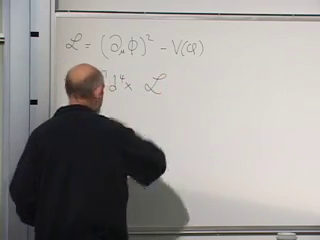
\includegraphics[width=0.78\textwidth]{lecture_01_figure_03.png}
\caption{La densité lagrangienne scalaire locale et son intégrale sur l’espace-temps, qui donne l’action.}
\lectureframe{00:26:08}
\end{figure}

La densité lagrangienne est locale : elle décrit un point de l’espace-temps. Les équations classiques du champ découlent de la stationnarité de l’action. En théorie quantique, cette même action intervient dans la phase de l’intégrale de chemin \(\exp(iS)\). Dans les deux approches, la dimension de \(S\) est déterminante. Si l’on rétablit \(\hbar\), la phase est \(\exp(iS/\hbar)\) ; après avoir posé \(\hbar=1\), \(S\) doit lui-même être sans dimension.

\begin{classroomqa}
\audiencequestion{L’action a-t-elle pour unité \(\hbar\) ?\lecturetimestamp{00:26:13}}
\lecturerresponse{Oui. Puisque \(\hbar\) a été posé égal à un, l’action est sans dimension dans ces unités. La mesure quadridimensionnelle est de dimension \(L^4\) ; la densité lagrangienne doit donc être de dimension \(L^{-4}\).}
\end{classroomqa}

Le terme cinétique fixe alors la dimension du champ :
\begin{align}
[S]&=1, & [\mathcal L]&=L^{-4},\\
[\partial_\mu]&=L^{-1}, &
[(\partial\phi)^2]&=L^{-2}[\phi]^2=L^{-4},\nonumber\\
&& [\phi]&=L^{-1}.
\label{eq:scalar-dimension}
\end{align}
Ce bref calcul déterminera le comportement ultraviolet de chaque diagramme qui suit.

Développons le potentiel sous la forme
\begin{equation}
V(\phi)=\frac{m^2}{2}\phi^2+g\phi^3+\lambda\phi^4+\cdots.
\label{eq:scalar-potential}
\end{equation}
Chaque terme doit être de dimension \(L^{-4}\). Puisque
\([\phi^n]=L^{-n}\),
\begin{equation}
[m^2]=L^{-2},
\qquad
[g]=L^{-1},
\qquad
[\lambda]=1.
\label{eq:coupling-dimensions}
\end{equation}
Le couplage quartique est sans dimension. De tels couplages sont particulièrement importants en renormalisation, car leur dépendance en échelle ne peut pas se déduire d’une simple puissance de la longueur.

\begin{classroomqa}
\audiencequestion{\(g\) a-t-il une dimension de masse ?\lecturetimestamp{00:29:52}}
\lecturerresponse{Oui. Le facteur \(\phi^3\) est de dimension \(L^{-3}\), tandis que la densité de potentiel doit être de dimension \(L^{-4}\). Par conséquent, \([g]=L^{-1}\), qui est une masse en unités naturelles.}
\end{classroomqa}

\section{Sommets et propagateur à courte distance}

Les règles de Feynman se construisent à partir des sommets et des propagateurs. Le terme \(g\phi^3\) donne un sommet à trois lignes, associé à un facteur proportionnel à \(g\) ; le terme \(\lambda\phi^4\) donne un sommet à quatre lignes, associé à un facteur proportionnel à \(\lambda\). Le terme quadratique donne une insertion locale à deux points. On peut la représenter par une particule qui arrive, est absorbée, puis réémise, avec un coefficient proportionnel à \(m^2/2\). Les normalisations numériques, les signes, les facteurs de \(i\) et les facteurs de symétrie sont délibérément omis : le cours cherche à dégager la dépendance en échelle, et non à calculer une section efficace.

Ces dessins ont une interprétation opérationnelle. Un sommet à trois points peut absorber deux quanta et en émettre un, ou représenter toute autre attribution de ses trois lignes liée par croisement. Un sommet à quatre points peut décrire deux particules entrantes et deux particules sortantes. La croix quadratique est bien un sommet à deux lignes, même si elle est normalement incorporée au propagateur libre. Nous l’indiquons parce que nous reconnaîtrons bientôt tout processus à deux points non résolu en le comparant à ce sommet.

Un propagateur relie deux points de l’espace-temps. Sa ligne ne signifie pas qu’une particule quantique a suivi une trajectoire classique rectiligne. Elle représente l’amplitude de créer une excitation du champ en \(x\) et de l’absorber ou de la détecter en \(y\) :
\begin{equation}
\Delta(x-y)=\langle0|\phi(y)\phi(x)|0\rangle.
\label{eq:position-propagator}
\end{equation}
Lisons l’expression de droite à gauche. L’action de \(\phi(x)\) sur le vide crée une composante à une particule en \(x\). L’action de \(\phi(y)\) sur le bra élimine la composante en \(y\). Leur élément de matrice dans le vide est l’amplitude de recouvrement entre la création au premier point et la détection au second. Les symboles \(x\) et \(y\) désignent des quadrivecteurs entiers, et non deux simples coordonnées cartésiennes.

Les états sont sans dimension physique, tandis que chaque champ apporte \(L^{-1}\). Par conséquent,
\begin{equation}
[\Delta]=L^{-2}.
\end{equation}
Pour un champ sans masse, il n’existe pas d’échelle de longueur intrinsèque ; l’analyse dimensionnelle impose donc le comportement à courte distance
\begin{equation}
\Delta(x-y)\sim\frac{1}{(x-y)^2}.
\label{eq:massless-propagator}
\end{equation}
Le dénominateur est la séparation au carré invariante de Lorentz, avec la prescription usuelle au voisinage de ses singularités.\editorialnote{Pour le décompte des puissances, il est commode de faire une rotation de Wick vers une séparation euclidienne, dont le module est sans ambiguïté proportionnel à \(1/|x-y|^2\). Cela ne modifie pas les puissances ultraviolettes utilisées ci-dessous.}

Lorsque \(y\) tend vers \(x\), le propagateur diverge. Cette singularité de propagation sur une séparation qui tend vers zéro est à l’origine des divergences ultraviolettes des diagrammes plus élaborés.

\section{Renormalisation de la masse d’un scalaire}

Pour un champ scalaire, le paramètre dynamique est \(m^2\), comme le suggère déjà la relation de dispersion relativiste :
\begin{equation}
E=\sqrt{\mathbf p^2+m^2}.
\end{equation}
Soit \(\delta\) la plus petite distance que notre description effective permet de résoudre. Nous ne distinguerons pas les processus dont les sommets sont séparés par une distance inférieure à \(\delta\). Tout processus non résolu de ce type, avec un scalaire entrant et un scalaire sortant, a la même structure observable à deux points qu’une insertion de masse ; il doit donc contribuer à la masse effective.

Considérons un accélérateur comme un microscope. Si sa résolution la plus fine est \(\delta\), une absorption en un point suivie d’une émission à une distance bien inférieure à \(\delta\) ne peut être distinguée d’un événement véritablement local. Nous floutons délibérément le sommet à cette échelle. La renormalisation est la règle qui transfère tous ces processus possibles, situés sous le seuil de résolution, dans le coefficient de l’opérateur local correspondant.

\subsection{Première correction quartique}

Commençons par un unique sommet \(\phi^4\). Deux lignes correspondent à la particule externe ; les deux autres se rejoignent pour former une petite boucle, émise puis réabsorbée presque au même point. En étalant le propagateur au point coïncident sur la distance de coupure, on obtient
\begin{equation}
\Delta(0)\ \longrightarrow\ \Delta(\delta)\sim\frac{1}{\delta^2},
\end{equation}
d’où
\begin{equation}
\delta m^2_{(1)}\sim\frac{\lambda}{\delta^2}.
\label{eq:one-loop-scalar-mass}
\end{equation}
Si \(m_0^2\) désigne le paramètre d’entrée, ou paramètre nu, le coefficient à deux points mesuré à basse résolution prend schématiquement la forme
\begin{equation}
\frac{m_{\mathrm{eff}}^2}{2}
\sim
\frac{m_0^2}{2}
+c_1\frac{\lambda}{\delta^2},
\label{eq:first-renormalized-mass}
\end{equation}
où \(c_1\) regroupe les facteurs numériques et les conventions omis. La masse mesurée en laboratoire dans des expériences qui ne résolvent pas les distances inférieures à \(\delta\) est cette quantité renormalisée, et non \(m_0\) à elle seule.

Il existe donc deux façons indiscernables de produire l’événement observé à deux points. Le sommet quadratique initial peut absorber puis réémettre la particule, ou bien l’interaction quartique peut le faire en émettant puis en réabsorbant brièvement un scalaire virtuel. En mécanique quantique, les amplitudes s’additionnent. Dès que la boucle se trouve sous le seuil de résolution, son histoire distincte disparaît de la description effective, mais sa contribution au coefficient mesuré demeure.

\subsection{Correction quartique suivante}

Relions maintenant deux sommets quartiques de sorte qu’une particule externe entre en \(x\), qu’une autre en sorte en \(x+\Delta\) et que trois propagateurs internes relient les sommets. On a deux puissances de \(\lambda\), tandis que les propagateurs apportent \(\Delta^{-6}\). Les amplitudes quantiques doivent être sommées sur tous les points non résolus d’où la particule sortante peut émerger ; on intègre donc sur le quadrivecteur relatif :
\begin{equation}
\delta m^2_{(2)}
\sim
\lambda^2
\int_{|\Delta|\gtrsim\delta}
d^4\Delta\,\frac{1}{|\Delta|^6}.
\label{eq:two-loop-power-count}
\end{equation}

\begin{classroomqa}
\audiencequestion{La petite marque au sommet signifie-t-elle qu’il n’y a que trois particules à cet endroit ?\lecturetimestamp{00:46:35}}
\lecturerresponse{Non. Nous utilisons toujours l’interaction quartique. Quatre lignes se rejoignent à chaque sommet ; dans ce diagramme à deux points, une ligne est externe et trois relient les deux sommets. Le second sommet a également quatre lignes incidentes.}
\end{classroomqa}

La mesure apporte quatre puissances de longueur et les trois propagateurs en apportent moins six. Puisque la coupure ultraviolette est la seule échelle de cette estimation,
\begin{equation}
\int_{|\Delta|\gtrsim\delta}
\frac{d^4\Delta}{|\Delta|^6}
\sim\frac{1}{\delta^2},
\qquad
\delta m^2_{(2)}
\sim\frac{\lambda^2}{\delta^2}.
\label{eq:two-loop-scalar-mass}
\end{equation}
Ici, \(\Delta^\mu\) est une variable d’intégration à quatre composantes ; on intègre sur sa composante temporelle et ses trois composantes spatiales. Le \(\delta\) minuscule désigne la coupure fixe. Le cours emploie d’abord le même nom oral pour les deux, puis rectifie la notation.

On retrouve le même résultat en exprimant radialement la mesure quadridimensionnelle. À une constante angulaire près,
\begin{equation}
\int_{\delta}\frac{d^4\Delta}{|\Delta|^6}
\sim
\int_{\delta}\frac{R^3\,dR}{R^6}
=\int_{\delta}\frac{dR}{R^3}
\sim\frac{1}{\delta^2}.
\end{equation}
C’est pourquoi la limite supérieure à grande distance n’a pas d’importance pour l’estimation ultraviolette : l’intégrale est dominée par son extrémité inférieure.

Les diagrammes d’ordre supérieur reproduisent le même schéma. Un diagramme avec davantage de sommets quartiques ajoute une puissance supérieure de \(\lambda\), mais l’analyse dimensionnelle autorise toujours une contribution quadratiquement divergente à la masse :
\begin{equation}
\begin{aligned}
m_{\mathrm{eff}}^2
={}&m_0^2
+\frac{1}{\delta^2}
\left(c_1\lambda+c_2\lambda^2+c_3\lambda^3+\cdots\right)\\
&+\text{weaker terms}.
\end{aligned}
\label{eq:scalar-mass-series}
\end{equation}

\subsection{Interaction cubique et logarithme}

Deux sommets cubiques donnent deux propagateurs entre des points proches. Leur contribution est proportionnelle à
\begin{equation}
\delta m_g^2
\sim
g^2\int_{|\Delta|\gtrsim\delta}
\frac{d^4\Delta}{|\Delta|^4}.
\label{eq:cubic-loop}
\end{equation}
Cette fois, la mesure et le dénominateur portent le même nombre de puissances. La dépendance restante est logarithmique plutôt qu’une puissance :
\begin{equation}
\delta m_g^2
\sim
c_g g^2\log\!\left(\frac{1}{\mu\delta}\right).
\label{eq:cubic-log}
\end{equation}
L’échelle de référence \(\mu\) rend le logarithme sans dimension. C’est la version entièrement dimensionnée de l’expression schématique \(g^2\log\delta\) du cours. Un logarithme varie beaucoup plus lentement que n’importe quelle puissance inverse ; ainsi, \(1/\delta^2\) domine lorsque la coupure correspond à une distance de plus en plus courte.

La forme radiale rend, là encore, la distinction évidente :
\begin{equation}
\int_{\delta}^{R_{\mathrm{IR}}}
\frac{d^4\Delta}{|\Delta|^4}
\sim
\int_{\delta}^{R_{\mathrm{IR}}}\frac{R^3\,dR}{R^4}
=\log\!\left(\frac{R_{\mathrm{IR}}}{\delta}\right).
\end{equation}
Quand les puissances de la mesure et du dénominateur sont égales, on obtient un logarithme. Si le dénominateur comporte davantage de puissances, on obtient une puissance inverse de la coupure. Le cours ne nous demande pas d’évaluer les facteurs angulaires ; il nous apprend à reconnaître immédiatement la réponse ultraviolette.

\begin{classroomqa}
\audiencequestion{Quelle base utilise-t-on pour le logarithme ?\lecturetimestamp{00:57:42}}
\lecturerresponse{On utilise le logarithme népérien. Un changement de base ne fait que le multiplier par une constante numérique, laquelle est absorbée dans le coefficient dont les facteurs de \(2\), de \(\pi\) et de symétrie n’ont pas été calculés ici.}
\end{classroomqa}

\begin{classroomqa}
\audiencequestion{Comment peut-on prendre le logarithme d’une longueur, et d’où viennent les unités de la correction de masse ?\lecturetimestamp{00:58:32}}
\lecturerresponse{Un logarithme compare toujours deux échelles ; il s’agit donc, rigoureusement, du logarithme d’un rapport sans dimension tel que \(1/(\mu\delta)\). Le couplage \(g\) a une puissance de masse ; \(g^2\) possède donc déjà exactement la dimension d’une masse au carré requise pour la correction.}
\end{classroomqa}

\begin{classroomqa}Un diagramme de Feynman donne une amplitude. Le carré de son module est-il une probabilité ?\audiencequestion{
\lecturetimestamp{00:59:41}}\lecturerresponse{Oui, lorsque l’amplitude intervient dans le calcul d’une transition physique avec les facteurs d’états et d’espace des phases requis. Ici, son rôle immédiat est différent : l’amplitude non résolue d’un processus à deux points a la même forme locale que le terme de masse et déplace donc le paramètre de masse effective.}
\end{classroomqa}

\section{Tous les paramètres deviennent effectifs}

La famille infinie de diagrammes de masse ne disparaît pas simplement parce que \(\lambda\) est petit. La théorie des perturbations les ordonne selon les puissances du couplage ; les termes successifs peuvent donc être de plus en plus petits, mais ils restent en nombre infini. L’élimination des courtes distances renormalise également les interactions elles-mêmes.

\begin{classroomqa}
\audiencequestion{Même pour la renormalisation de la masse, n’y a-t-il pas une infinité de diagrammes ?\lecturetimestamp{01:00:35}}
\lecturerresponse{Si. Si \(\lambda\) est suffisamment petit, la série perturbative peut être utile, car les puissances supérieures sont successivement supprimées. Néanmoins, le paramètre renormalisé est défini par la série entière, et non par le seul premier diagramme.}
\end{classroomqa}

Sur le plan opérationnel, une interaction locale \(\lambda\phi^4\) est une amplitude à deux particules entrantes et deux particules sortantes. Si un processus à quatre points plus complexe se déroule entièrement dans une région non résolue, il est indiscernable, à basse résolution, du sommet local initial. Ces diagrammes sont donc regroupés dans un \(\lambda\) effectif. En quatre dimensions, leur dépendance dominante en échelle est généralement logarithmique dans la théorie \(\phi^4\). Le cours ne calcule pas cette fonction bêta ; il se sert de cet exemple pour énoncer le principe général :
\begin{equation}
\begin{gathered}
\text{parameters measured at low energy}\\
\ne\\
\text{parameters entered at the microscopic cutoff}
\end{gathered}
\end{equation}

L’exemple à quatre points est important, car il écarte un possible malentendu. La renormalisation n’est pas une réparation spéciale appliquée uniquement à une divergence de masse. Tout opérateur autorisé dans le lagrangien peut être reproduit par des diagrammes non résolus ayant les mêmes lignes externes et les mêmes symétries. Un processus à deux points renormalise un coefficient quadratique, un processus à quatre points renormalise un coefficient quartique, et les processus du vide au vide renormalisent le terme constant. Le lagrangien à basse énergie est le registre concis où sont consignés tous ces processus à courte distance.

\begin{classroomqa}
\audiencequestion{Puisque \(\Delta\) a pour unité une longueur, prendre son logarithme n’est-il pas dimensionnellement étrange ? Et le tableau a-t-il interverti delta majuscule et delta minuscule ?\lecturetimestamp{01:01:34}}
\lecturerresponse{Le logarithme désigne en réalité le rapport à une autre échelle ; il est donc sans dimension. Oui, la notation a été brièvement intervertie : \(\Delta^\mu\) est la variable d’intégration, tandis que \(\delta\) est la coupure de distance inférieure qui subsiste dans le résultat.}
\end{classroomqa}

C’est l’équivalent, en théorie des champs, du cas de la molécule. Nous avons résolu le mouvement des électrons rapides, invisibles, puis intégré leur résultat dans un potentiel. Ici, nous faisons la somme des processus invisibles à courte distance et intégrons leur résultat dans les masses, les couplages et tous les autres coefficients locaux autorisés. Tous les paramètres sont décalés.

\begin{classroomqa}
\audiencequestion{Pourriez-vous répéter si la quantité mesurée inclut les échelles plus petites que celles que l’expérience peut voir ?\lecturetimestamp{01:05:13}}
\lecturerresponse{Oui. Les fluctuations individuelles ne sont pas résolues, mais leur effet cumulé est présent. Tous les diagrammes qui font intervenir des échelles plus courtes sont regroupés dans un unique coefficient effectif, que l’expérience à basse énergie interprète par exemple comme la masse au carré physique.}
\end{classroomqa}

\begin{classroomqa}
\audiencequestion{Le terme d’entrée \(m_0^2\) doit-il alors annuler les autres contributions ?\lecturetimestamp{01:06:00}}
\lecturerresponse{Si la masse scalaire mesurée est bien plus petite que les contributions ultraviolettes prises individuellement, oui. Cette annulation nécessaire est le problème du réglage fin que nous allons maintenant aborder.}
\end{classroomqa}

\section{Le problème de la hiérarchie du Higgs}

Imaginons que la coupure soit la longueur de Planck, de sorte que la théorie effective des champs doit résumer les fluctuations depuis les échelles de laboratoire jusqu’à l’échelle où la gravité quantique doit intervenir. En unités de physique des particules,
\begin{equation}
\delta\sim M_{\mathrm{Pl}}^{-1}\sim10^{-19}\,\mathrm{GeV}^{-1},
\qquad
\frac{1}{\delta^2}\sim10^{38}\,\mathrm{GeV}^2.
\label{eq:planck-cutoff}
\end{equation}
Le choix précis entre l’échelle de Planck réduite et non réduite ne change rien à l’énormité de l’écart.

La hiérarchie des distances est tout aussi frappante. La longueur de Planck est environ dix-neuf ordres de grandeur inférieure au rayon du proton, et environ seize ou dix-sept ordres de grandeur inférieure aux distances directement sondées par les accélérateurs évoqués ici. Le fait d’élever cet écart au carré conduit à l’annulation d’environ trente-quatre ordres de grandeur dans un paramètre de masse scalaire au carré.

Pour le champ de Higgs, qui est un scalaire, l’échelle faible recherchée est de l’ordre de quelques centaines de GeV, et non de \(10^{19}\) GeV. Pourtant, les termes de l’équation~\eqref{eq:scalar-mass-series} peuvent naturellement être de l’ordre de l’échelle de Planck.
Leurs signes n’ont pas été suivis : certains peuvent être positifs, d’autres négatifs, et la masse au carré nue peut elle aussi avoir l’un ou l’autre signe. Mais, pour laisser un résidu à l’échelle électrofaible, ces contributions énormes doivent s’annuler à environ trente-quatre chiffres après la virgule. Susskind commence par dire dix-sept chiffres, puis se corrige, car la comparaison porte sur des masses au carré. C’est le rapport au carré qui mesure ce réglage dans ce cas.

\begin{classroomqa}
\audiencequestion{\(\lambda\) est-il inférieur ou supérieur à un ?\lecturetimestamp{01:09:50}}
\lecturerresponse{On suppose qu’il est légèrement inférieur à un. La théorie des perturbations deviendrait inextricable si les puissances successives augmentaient, et une théorie purement scalaire ne peut pas non plus être extrapolée de manière cohérente avec un couplage quartique arbitrairement grand. Mais \(\lambda\) est loin d’être aussi petit que \(10^{-38}\) ; pour se repérer, le cours retient une valeur de l’ordre du pour cent.}
\end{classroomqa}

\begin{classroomqa}
\audiencequestion{Même si \(\lambda<1\), ne reste-t-il pas beaucoup de termes importants, puisque chacun comporte le grand facteur de coupure ?\lecturetimestamp{01:10:43}}
\lecturerresponse{Oui. Les puissances élevées finissent par supprimer la série, mais un grand nombre de termes peuvent contribuer avant que cela ne se produise. Ces termes et le terme nu devraient tous se compenser de façon à ne laisser que la valeur physique extraordinairement petite.}
\end{classroomqa}

Rappelons pourquoi l’on sait que le paramètre de masse du boson de Higgs est à l’échelle électrofaible. Avec les conventions du cours, écrivons le potentiel de brisure de symétrie sous la forme
\begin{equation}
V(\phi)=-\frac{\mu^2}{2}\phi^2+\frac{\lambda}{4}\phi^4.
\label{eq:higgs-potential}
\end{equation}
Le coefficient quadratique négatif rend l’origine instable, tandis que le terme quartique positif stabilise le potentiel. En dérivant,
\begin{equation}
\frac{dV}{d\phi}=-\mu^2\phi+\lambda\phi^3
=\phi(-\mu^2+\lambda\phi^2),
\end{equation}
on obtient le minimum non nul
\begin{equation}
\phi_{\min}^2=f^2=\frac{\mu^2}{\lambda}.
\label{eq:higgs-minimum}
\end{equation}
Le tableau écrit le terme quartique de façon schématique sous la forme \(\lambda\phi^4\), mais cite l’équation ~\eqref{eq:higgs-minimum} ; l’insertion du facteur conventionnel \(1/4\) rend ces deux lignes cohérentes sans modifier l’argument.

Le signe de \(-\mu^2\) est important, mais ne résout pas le problème de naturalité. C’est la courbure négative à l’origine qui entraîne la brisure spontanée de symétrie. La renormalisation modifie cette courbure par de grandes contributions positives et négatives. Pour obtenir le vide brisé observé, leur somme doit non seulement être petite, mais prendre la valeur négative précise qui place le minimum à l’échelle électrofaible.

Les masses des bosons \(W\) et \(Z\) déterminent \(f\) comme étant de l’ordre de \(200\,\mathrm{GeV}\) selon la normalisation approximative utilisée dans le cours. Si \(\lambda\) n’est ni énorme ni extraordinairement petit, \(\mu\) doit être du même ordre général. Le coefficient observé à l’échelle électrofaible est donc le résidu de contributions qui peuvent chacune être supérieures de plusieurs dizaines d’ordres de grandeur.

On appelle cela le problème du réglage fin du boson de Higgs, le problème de la hiérarchie ou le problème de la hiérarchie de jauge. La hiérarchie est le rapport immense entre l’échelle électrofaible ordinaire et une éventuelle échelle d’unification ou de Planck. Un petit nombre n’est pas en soi paradoxal. Ce qui est troublant ici, c’est qu’un petit nombre résulte de contributions importantes, apparemment sans rapport, qui doivent s’annuler avec une extrême précision. Le problème a été reconnu à la fin des années 1970 et au début des années 1980, et la recherche d’un mécanisme à l’origine de cette annulation motive la supersymétrie ainsi que plusieurs idées concurrentes.

La série perturbative infinie aiguise le problème au lieu de le résoudre. Une valeur de \(\lambda\) de l’ordre du pour cent rend suffisamment petites les puissances assez élevées, mais de nombreux termes peuvent apparaître avant que cette suppression ne l’emporte. Il ne suffit pas qu’une boucle annule fortuitement la masse nue. L’échelle électrofaible effective doit rester stable après inclusion du reste des processus à courte distance. Une relation structurelle entre les termes fournirait une explication ; une annulation chiffre par chiffre entre des contributions sans rapport ne constitue qu’un réglage fin.

\section{Pourquoi la masse d’un fermion se comporte mieux}

Les autres particules du Modèle standard ne nécessitent pas de réglages fins indépendants du même type. Pour un fermion de Dirac, le terme de masse est
\begin{equation}
\mathcal L_m=-m\bar\psi\psi
=-m\left(\bar\psi_L\psi_R+\bar\psi_R\psi_L\right).
\label{eq:fermion-mass}
\end{equation}
Il contient la masse, et non son carré, et couple les chiralités gauche et droite. Une insertion locale de masse transforme donc \(L\) en \(R\), ou \(R\) en \(L\).

\begin{figure}[htbp]\centering
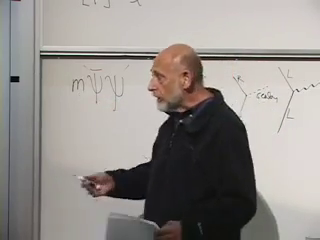
\includegraphics[width=0.76\textwidth]{lecture_01_figure_04.png}\caption{Le terme de masse du fermion et les schémas tracés au tableau illustrant les changements de chiralité. Les diagrammes sont reconstitués algébriquement ci-dessous, car une partie du travail à la craie est masquée.}\lectureframe{01:23:36}\end{figure}

Dans le cours oral, il est souvent question de caractère droitier ou de l’hélicité. La protection exacte s’énonce le plus clairement en termes de chiralité. Pour une particule ultrarelativiste, l’image fondée sur l’hélicité donne l’intuition recherchée, mais la chiralité est la grandeur portée par les champs gauches et droits dans l’équation ~\eqref{eq:fermion-mass}.

Les interactions de jauge préservent la chiralité :
\begin{equation}
L\xrightarrow{\ \gamma\ }L,
\qquad
R\xrightarrow{\ \gamma\ }R.
\label{eq:gauge-preserves-chirality}
\end{equation}
Une interaction de Yukawa avec un scalaire relie des chiralités opposées :
\begin{equation}
L\xleftrightarrow{\ \phi\ }R.
\label{eq:scalar-flips-chirality}
\end{equation}
Supposons d’abord que l’électron soit initialement dans l’état \(m_0=0\). L’émission puis la réabsorption d’un nombre quelconque de photons ne peuvent pas produire de masse, car chaque vertex de jauge préserve la chiralité. Une suite d’interactions qui commence à gauche reste à gauche. L’électrodynamique quantique pure permet donc de manière cohérente un électron sans masse : son auto-énergie électromagnétique ne peut pas engendrer une masse additive à partir de zéro.

Dans le schéma de lignes, partons d’un électron de chiralité gauche. Au premier vertex photonique, sa chiralité est toujours gauche ; après la propagation et la réabsorption du photon, elle est encore gauche. Répéter cette construction ne fait qu’insérer davantage de vertex qui préservent la chiralité. La fonction à deux points externe peut être renormalisée, mais elle ne peut pas acquérir la structure gauche-droite qui définit une masse.

L’émission d’un scalaire pourrait-elle y parvenir ? Un vertex scalaire transforme \(L\) en \(R\), mais le scalaire émis doit être réabsorbé. Un graphe d’auto-énergie à deux points contient donc un nombre pair de vertex scalaires. Le second changement de chiralité inverse le premier, si bien que le graphe complet préserve à nouveau la chiralité externe. Quelle que soit la complexité du graphe interne, l’appariement des vertex par émission et réabsorption empêche l’apparition d’un terme de \(L\) à \(R\) additif lorsque la masse initiale est nulle.

Il s’agit d’un argument de parité sur le nombre de changements de chiralité. Un vertex scalaire change la chiralité une fois ; la fermeture de chaque ligne scalaire interne exige une seconde extrémité, et donc un second changement de chiralité. Quatre vertex scalaires entraînent quatre changements, et ainsi de suite. Un nombre pair ramène le fermion à sa chiralité initiale. Cette conclusion ne se limite pas à la boucle la plus simple dessinée au tableau.

Une correction de masse non nulle n’est possible que si le diagramme contient déjà une insertion de masse. Par exemple, l’émission et la réabsorption d’un photon peuvent encadrer une insertion de \(m_0\bar\psi\psi\). Les vertex de jauge apportent deux puissances de la charge électrique, mais le seul changement de chiralité apporte la masse initiale :
\begin{equation}
\begin{aligned}
m_e
&=m_0+c_1e^2m_0+c_2e^4m_0+\cdots\\
&=m_0\left(1+c_1e^2+c_2e^4+\cdots\right).
\end{aligned}
\label{eq:multiplicative-fermion-mass}
\end{equation}
Si \(m_0=0\), le résultat reste nul. Si \(m_0\) est petit, chaque correction est proportionnelle à ce petit nombre. On peut toujours se demander pourquoi l’électron est léger par rapport à une échelle fondamentale, mais on n’a plus à soustraire de grandes quantités sans rapport pour l’obtenir. En ce sens, une faible masse de fermion est techniquement naturelle.

L’insertion de masse explicite la séquence autorisée. Partons de \(L\). L’émission d’un photon préserve \(L\) ; l’insertion \(m_0\) transforme \(L\) en \(R\) ; la réabsorption du photon préserve \(R\). Le diagramme possède maintenant la chiralité externe d’un terme de masse, mais sa valeur comporte nécessairement le facteur \(m_0\). C’est là le contraste crucial avec l’équation ~\eqref{eq:one-loop-scalar-mass}, dont la correction scalaire reste non nulle même lorsque la masse scalaire initiale est fixée à zéro.

Les bosons de jauge bénéficient d’une protection analogue : la symétrie de jauge interdit un terme de masse indépendant, de sorte qu’un boson de jauge initialement sans masse le reste à tous les ordres perturbatifs. Dans le Modèle standard, les masses des fermions et des bosons de jauge faibles apparaissent en réponse à la valeur moyenne dans le vide du champ de Higgs. Si l’échelle du Higgs est maîtrisée, les autres masses légères n’exigent pas de reproduire séparément le même réglage fin catastrophique.

Cela précise la question à laquelle la supersymétrie entend répondre : une théorie peut-elle empêcher le scalaire de Higgs de recevoir une correction de masse additive énorme ? La réponse est oui dans des cadres supersymétriques appropriés, parce que les contributions bosoniques et fermioniques sont liées plutôt qu’indépendantes. Le mécanisme détaillé sera abordé dans le cours suivant.

\section{L’autre réglage fin : l’énergie du vide}

Il existe un problème de renormalisation encore plus grave, mais il ne devient observable que lorsque l’on inclut la gravité. En physique non gravitationnelle, ajouter une constante à toutes les énergies ne modifie aucune expérience. La masse de l’électron, par exemple, n’est pas une énergie absolue ; c’est l’énergie supplémentaire nécessaire pour ajouter un électron au vide :
\begin{equation}
m_e=E(\text{vacuum}+\text{one electron})-E(\text{vacuum})
\end{equation}
dans le référentiel de repos de l’électron. Si le vide et tous les états excités sont décalés de la même façon, leurs différences restent inchangées.

Les diagrammes du vide au vide modifient néanmoins l’énergie du vide. Dans la théorie \(\lambda\phi^4\), réunissons les quatre pattes d’un vertex quartique en deux boucles courtes. Chaque propagateur pris au même point fournit \(1/\delta^2\), donc
\begin{equation}
\delta\rho_{\mathrm{vac}}
\sim
c_{\mathrm{vac}}\frac{\lambda}{\delta^4}.
\label{eq:vacuum-energy-divergence}
\end{equation}
Les diagrammes du vide plus complexes comportent d’autres facteurs de couplage et coefficients, mais l’analyse dimensionnelle donne généralement la même dépendance quartique à la coupure pour une densité d’énergie.

L’absence de lignes externes identifie précisément la correction. Les graphes à deux points comparent un état à une particule au vide et modifient une masse ; les graphes à quatre points modifient la diffusion ; un graphe sans particules entrantes ni sortantes modifie l’amplitude du vide au vide elle-même. Un vertex quartique fournit \(\lambda\), et ses deux boucles courtes fournissent chacune \(\delta^{-2}\). L’analyse dimensionnelle impose alors l’échelle de densité d’énergie \(\delta^{-4}\).

Sans gravité, on peut choisir le zéro de l’énergie et se demander à qui cela importe. La relativité générale supprime cette liberté : le tenseur énergie-impulsion est une source de la courbure de l’espace-temps, si bien qu’une énergie uniforme du vide fait graviter l’espace vide. Elle apparaît sous la forme d’une constante cosmologique et est reliée, du point de vue observationnel, à l’énergie noire. Une énergie du vide mesurée comme infime doit alors subsister malgré des contributions de la forme \(\delta^{-4}\).

Voilà pourquoi la question change lorsqu’on introduit la gravité. En mécanique quantique ordinaire, décaler tous les niveaux d’une même constante ne modifie aucune fréquence de transition. En gravité, cette constante n’est pas inerte : le tenseur de contrainte du vide est proportionnel à la métrique et courbe l’espace-temps. Ce qui était un zéro arbitraire de l’énergie devient une source dans l’équation d’Einstein.

Il existe donc au moins deux problèmes de naturalité extrêmes. Le cours évoque environ 123 décimales de réglage fin pour l’énergie du vide et environ 30--35 pour la masse du Higgs. Les nombres exacts dépendent de l’échelle ultraviolette et des conventions, mais le contraste ne fait aucun doute. La supersymétrie est une réponse possible au problème du Higgs abordé ici ; une fois brisée, elle n’explique pas à elle seule la constante cosmologique observée.\editorialnote{C’est aussi pourquoi une annulation exacte boson--fermion ne constitue pas une solution phénoménologique à l’énergie du vide observée : la supersymétrie doit être brisée dans notre monde.}

\section{Questions de fin de cours}

\begin{classroomqa}
\audiencequestion{La correction au Higgs dépend de la coupure \(\delta\), mais celle-ci semble arbitraire. Pourrait-elle correspondre à la longueur de Planck, à dix fois la longueur de Planck ou à autre chose ? Cela rend-il le réglage fin arbitraire ?\lecturetimestamp{01:33:50}}
\lecturerresponse{La contribution numérique dépend de l’échelle la plus courte jusqu’à laquelle on peut faire confiance à la théorie effective. Cette dépendance relève du bilan physique, elle ne permet pas d’échapper au problème. Les modes jusqu’à toute échelle où le Modèle standard reste valable sont des modes dont il faut inclure les effets. Choisissons \(\delta\) à la distance où l’on s’attend à ce qu’une nouvelle physique apparaisse---peut-être l’échelle de Planck, peut-être une échelle d’unification proche de \(10^{16}\,\mathrm{GeV}\). La contribution accumulée jusqu’à cette échelle constitue déjà une borne inférieure du problème. Prolonger la même théorie jusqu’à des distances encore plus courtes ne fait qu’accroître la dépendance quadratique. Nous devons expliquer ce qui annule la contribution provenant de chaque échelle entre le laboratoire et cette limite ultraviolette.}
\end{classroomqa}

\begin{classroomqa}
\audiencequestion{Qu’est-ce qui définit une particule scalaire, et quel en est un exemple ?\lecturetimestamp{01:37:26}}
\lecturerresponse{Le Higgs est l’exemple visé. Un scalaire ne se transforme pas en différentes composantes sous une rotation spatiale ; de manière équivalente, ses quanta ont un spin nul. Le photon est décrit par un champ vectoriel, et le champ gravitationnel par un tenseur. À l’époque de cette conférence 2010, aucune particule élémentaire de spin nul n’avait encore été détectée.\editorialnote{Le boson de Higgs a été découvert au CERN en 2012 et ses propriétés mesurées sont compatibles avec un spin nul.}}
\end{classroomqa}

\begin{classroomqa}
\audiencequestion{La particule \(Z\) est-elle aussi un boson de jauge ?\lecturetimestamp{01:38:31}}
\lecturerresponse{Oui. Les \(Z\), \(W^+\) et \(W^-\) sont des bosons de jauge de spin un, tout comme le photon. Leurs équations de champ et leurs interactions sont des généralisations non abéliennes ou électrofaibles de la description de jauge de type Maxwell.}
\end{classroomqa}

\begin{classroomqa}
\audiencequestion{Pourquoi la contribution de l’état fondamental bosonique ne s’annule-t-elle pas avec la contribution fermionique dans l’énergie du vide ?\lecturetimestamp{01:39:10}}
\lecturerresponse{Les boucles de fermions et les boucles bosoniques correspondantes peuvent effectivement contribuer avec des signes opposés. L’annulation n’est toutefois pas automatique : les masses, les multiplicités et les couplages des particules doivent correspondre. Même un faible désaccord laisse un résidu important dépendant de la coupure, et les familles infinies de diagrammes doivent correspondre ordre par ordre. La supersymétrie exacte impose précisément de telles relations boson--fermion. Le contenu générique en particules d’une théorie non supersymétrique ne les impose pas, et une supersymétrie brisée laisse subsister un problème d’énergie du vide.}
\end{classroomqa}

\section{Mise en perspective}

Le parcours du cours suit un enchaînement délibéré. Un calcul moléculaire montre d’abord que l’élimination des variables rapides n’est ni une négligence ni un tour de magie : leur énergie d’état fondamental devient un potentiel pour les variables lentes. La théorie quantique des champs répète cette opération à différentes longueurs d’onde. L’analyse dimensionnelle révèle ensuite quels paramètres effectifs sont sensibles à la coupure. Les masses scalaires reçoivent des termes additifs proportionnels à \(\delta^{-2}\) ; l’échelle du Higgs, lorsqu’elle est faible, semble donc d’une fragilité contre nature. Les masses des fermions sont renormalisées multiplicativement, car la chiralité protège la limite de masse nulle ; la symétrie de jauge protège de même les bosons de jauge sans masse. L’énergie du vide est encore plus sensible et varie comme \(\delta^{-4}\) ; la gravité rend sa valeur absolue observable.

La supersymétrie intervient dans le cours précisément à ce stade, non comme un ornement mathématique, mais comme une tentative de faire se comporter le secteur scalaire davantage comme les secteurs protégés. L’étape suivante consiste à comprendre quelle symétrie peut relier les bosons et les fermions assez étroitement pour organiser ces annulations.
